\documentclass[11pt]{article}
\usepackage[T1]{fontenc}
\usepackage{lmodern,amsmath,amssymb,amsthm,booktabs,array,graphicx,microtype}
\usepackage[letterpaper,margin=1in]{geometry}
\usepackage[dvipsnames]{xcolor}
\usepackage[colorlinks=true,linkcolor=MidnightBlue,citecolor=MidnightBlue,urlcolor=MidnightBlue,
  pdftitle={Normality of localized logarithms and polylogarithms on finite prime supports}]{hyperref}
\newtheorem{theorem}{Theorem}[section]
\newtheorem{lemma}[theorem]{Lemma}
\newtheorem{corollary}[theorem]{Corollary}
\newtheorem{proposition}[theorem]{Proposition}
\newcommand{\Z}{\mathbb Z}
\newcommand{\Q}{\mathbb Q}
\newcommand{\R}{\mathbb R}
\newcommand{\N}{\mathbb N}
\newcommand{\vol}{\lambda}
\newcommand{\dd}{D_{\infty}}
\newcommand{\fract}[1]{\{#1\}}
\newcommand{\den}{\operatorname{den}}
\newcommand{\repo}{https://github.com/eldernos/MathematicsResearch}
\newcommand{\sha}{a09e011720bc74396a27f4cb3ce2d8a5b3ce5035}
\newcommand{\decl}[3]{\href{\repo/blob/\sha/NormalityChecker/#1.lean\#L#2}{\texttt{\detokenize{#3}}}}
\setlength{\emergencystretch}{1em}
\title{Normality of localized logarithms and polylogarithms\\on finite prime supports}
\author{}
\date{}
\begin{document}
\maketitle
\begin{abstract}
Let \(M(S)\) consist of the positive integers generated by a finite set \(S\) of primes. For integers \(b\ge2\) and \(s\ge1\), the base-\(b\) interval discrepancy of \(\sum_{m\in M(S)}m^{-s}b^{-m}\) tends to zero if some \(p\in S\) does not divide \(b\), and to one otherwise. For a nonzero polynomial \(P\in\Q[X]\), the corresponding series with numerator \(P(m)\) is normal precisely when \(P(X)/X^s\) has a pole at zero and such a prime exists. We prove that persistent cancellation at a single off-radix prime has measure zero by taking multiplicative differences on a logarithmic circle and separating the remaining thresholds. At each cutoff the discrepancy differs by \(o(1)\) from the proportion of simultaneous persistent failures at all off-radix primes and all orders up to \(s\). For restrictions of the support we give bounds in terms of retained prime powers and a complete criterion on one prime-power axis.
\end{abstract}

\section{The classifications}
For a finite set \(S\) of primes put \(M(S)=\{m\ge1:p\mid m,\ p\ \text{prime}\Rightarrow p\in S\}\). In particular \(M(\varnothing)=\{1\}\). Given integers \(b\ge2\) and \(s\ge0\), \(P\in\Q[X]\), and \(A\subseteq M(S)\), write
\begin{equation}\label{eq:series}
 X_A(P,s)=\sum_{m\in A}\frac{P(m)}{m^s b^m},\qquad
 X_s=X_{M(S)}(1,s),\qquad J=\{p\in S:p\nmid b\}.
\end{equation}
Polynomial growth of the coefficients gives absolute convergence for every \(A\). At \(s=1\), \(X_1\) localizes the positive-coefficient series for \(-\log(1-b^{-1})\); positive \(s\) similarly localizes \(\operatorname{Li}_s(b^{-1})\).

Write \(\{y\}=y-\lfloor y\rfloor\). For \(0\le a<c\le1\) and \(N\ge1\) put
\[
 f_N(x;[a,c))=\frac1N\#\{0\le n<N:a\le\fract{b^nx}<c\},\qquad
 D_N(x)=\sup_{a,c}|f_N(x;[a,c))-(c-a)|.
\]
We use \(\dd(x)=\limsup_{N\to\infty}D_N(x)\). Normality in radix \(b\) means that every word of length \(k\ge1\) has limiting frequency \(b^{-k}\) at overlapping starting positions, using terminating expansions at radix rationals. A word specifies a half-open interval \([j/b^k,(j+1)/b^k)\). Convergence \(D_N\to0\) implies all these frequencies; conversely each interval is bracketed by unions of cylinders at one depth with length difference at most \(2b^{-k}\). The maximum error over the finitely many such unions tends to zero at each fixed \(k\). Thus normality is equivalent to \(D_N\to0\).

\begin{theorem}[Unsigned finite supports]\label{thm:unsigned}
For every finite prime set \(S\), integer \(b\ge2\) and integer \(s\ge1\),
\[
 \lim_{N\to\infty}D_N(X_s)=
 \begin{cases}0,&J\ne\varnothing,\\1,&J=\varnothing.\end{cases}
\]
In particular \(X_s\) is normal in radix \(b\) exactly when \(J\ne\varnothing\).
\end{theorem}

\begin{theorem}[Rational polynomial weights]\label{thm:polynomial}
Let \(P\in\Q[X]\setminus\{0\}\), let \(r\) be its order of vanishing at zero, and take \(s\ge0\). Then \(X_{M(S)}(P,s)\) is normal in radix \(b\) if and only if \(r<s\) and \(J\ne\varnothing\). If \(r\ge s\) or \(J=\varnothing\), every restriction \(X_A(P,s)\) is nonnormal. If \(D\) is a positive common denominator of the coefficients of \(P\) and \(D_0\) its largest divisor prime to \(b\), then in these cases
\[
 \liminf_{N\to\infty} D_N(X_A(P,s))\ \ge\ 1/D_0 .
\]
In particular the limit is one for integral \(P\).
\end{theorem}

The coefficient \(P(0)\) may be negative, and there is no upper bound on \(\deg P\). The zero polynomial, excluded in Theorem~\ref{thm:polynomial}, gives \(x=0\) and \(D_N=1\). With empty support the full sum is \(P(1)/b\). Figure~\ref{fig:matrix} records several instances of Theorem~\ref{thm:unsigned}. At \(b=10,\ S=\{2,3,5\}\) the single prime 3 suffices in every positive order despite both radix primes occurring in \(S\).

\begin{figure}[ht]
\centering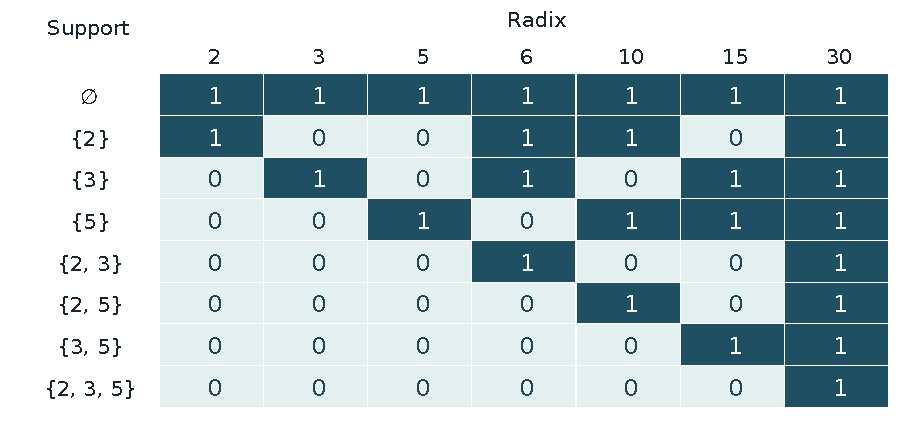
\includegraphics[width=.77\linewidth]{figures/classification.pdf}
\caption{Limit of the unsigned interval discrepancy for the indicated full supports and radices, at each integer order \(s\ge1\). Zero denotes normality. Each entry follows from divisibility by the radix (Theorem~\ref{thm:unsigned}).}\label{fig:matrix}
\end{figure}

\paragraph{Earlier results.}
Dibag introduced the localized logarithm in work on generalized Bernoulli coefficients \cite{dibag}. For a singleton \(S=\{p\}\) and \(p\nmid b\), the order-one sum differs by \(1/b\) from the standard Stoneham constant with parameter \(p\) \cite{stoneham}. Bailey and Crandall proved normality for all coprime Stoneham parameters \cite[Cor.~4.9]{bc}. Vandehey's fixed-prime exponential-sum estimate \cite[Cor.~1.2]{vandehey} supplies the short rational-orbit estimate used below. His normal-number construction \cite[Thm.~7.4]{vandehey} also covers the unsigned series at every positive order on any infinite subset of a single off-radix prime-power axis: the denominators \(c_i=p^{sk_i}\) form a divisibility chain and the insertion gaps at \(m_i=p^{k_i}\) are at least \((1-1/p)m_i\). Thus \(\exp((1+\epsilon)\log c_i/\log\log c_i)=o(m_i-m_{i-1})\) for fixed \(s,\epsilon>0\).

The 2026 manuscript \cite[Thms.~1.1, 4.1 and 5.1]{localized} proves binary normality on \(\{2,3\}\) at order one, with discrepancy \(O(N^{-1/2}\log^3(2N))\). Its finite-support extension covers nonempty sets wholly prime to \(b\), and all binary supports containing~3, at order one. The earlier rate is quantitative in this special case; the present classification gives convergence without a general rate. The accompanying Lean development in \cite{localized} covers the qualitative binary \(\{2,3\}\) result. Theorems~\ref{thm:unsigned} and~\ref{thm:polynomial} allow arbitrary overlap with the radix factors, all positive orders and, in the second theorem, rational polynomial numerators of unrestricted degree. On a support containing distinct primes \(p,q\), the ordered list of smooth indices contains both \(p\) and \(q\); their powers \(p^s,q^s\) cannot belong to one divisibility chain.

No uniformity in \(S\) is asserted. In the unrestricted logarithm every positive index contributes, whereas our count of exceptional digit positions uses the sparsity of \(M(S)\) for fixed \(S\). In particular these theorems do not decide binary normality of \(\log 2\).

\section{Rational orbits between insertions}
Write \(a_m=P(m)/m^s\) on \(A\) and zero elsewhere, and set \(R_n=\sum_{1\le m\le n}a_m b^{n-m}\). For the unsigned full support use \(R_{s,n}\). If \((n,n+i]\) contains no insertion, \(R_{n+i}=b^iR_n\). In the unsigned case
\begin{equation}\label{eq:tail}
 0\le b^nX_s-R_{s,n}\le (n+1)^{-s}/(b-1).
\end{equation}
For a polynomial numerator the shifted tail can grow immediately before an insertion.

\begin{lemma}[Transfer on intervals without insertions]\label{lem:transfer}
At each cutoff \(N\) one can discard \(o(N)\) positions and partition the rest into blocks \([u,u+B)\) of length \(B=\lfloor\sqrt N\rfloor\). On these blocks the following hold uniformly as \(N\to\infty\).
\begin{enumerate}
\item \(R_{u+i}=b^i R_u\) for \(0\le i<B\), and \(b^{u+i}X_A(P,s)-R_{u+i}=o(1)\).
\item The reduced denominator \(q_u=\den(R_u)\) has prime factors in a fixed finite set prime to \(b\), and \(q_u\le B^C\) for a fixed \(C\).
\item For every \(\varepsilon>0\) there exist \(N_0,Q_0\) such that on every retained block with \(N\ge N_0\) and \(q_u\ge Q_0\), the discrepancy of its \(B\) shifts is at most \(\varepsilon\).
\end{enumerate}
\end{lemma}
\begin{proof}
The number of smooth integers up to \(Y\) is at most \((1+\lfloor\log_2 Y\rfloor)^{|S|}\), by their exponent vectors. Partition \([0,N)\) at multiples of \(B\). Omit the initial block, the final remainder and each block with a smooth integer in \([u-B,u+2B]\). Each such integer up to \(N+2B\) removes at most four blocks. The discarded length is \(O(B(1+\log N)^{|S|})=o(N)\). With \(|a_m|\le K(m+1)^e\), the error at a retained position \(n\) is bounded by
\[
 K (n+B+2)^e b^{-B-1}\sum_{j\ge0}(1+j)^e b^{-j}=o(1).
\]
Here the next \(B\) positions contain no insertion.

Let \(c=\prod_{p\in J}p\) and \(H=\lceil\log_2(N+2B)\rceil\). Every contributing \(m\le u\) satisfies \(m^s\mid b^{sH}c^{sH}\). Split the coefficient denominator \(D=D_bD_0\) with \(D_b\mid b^\ell\) and \((D_0,b)=1\). Since \(u-m\ge B>sH+\ell\) eventually, the denominator of each shifted summand divides \(D_0 c^{sH}\). This is a common denominator with the asserted support and growth.

For a fixed integer \(h\ne0\), \(\den(hR_u)\ge q_u/|h|\). With \(q=\den(hR_u)\) the fixed-support orbit theorem gives
\(\big|\sum_{i<B}\exp(2\pi i h b^iR_u)\big|=o(B)\) uniformly when \(q\to\infty\) and \(q\le B^C\). This is the polynomial-length consequence of \cite[Cor.~1.2 in the preprint]{vandehey} for the fixed denominator primes. The error in the mean after replacing \(b^iR_u\) by \(b^{u+i}X_A(P,s)\) is at most \(2\pi |h|\) times the uniform tail bound. For any sequence of these blocks each nontrivial Fourier coefficient of its empirical measure therefore tends to zero. Approximation by trigonometric polynomials gives weak convergence to Lebesgue measure on the circle. Applying this to intervals with endpoints on a fixed finite grid and bounding an arbitrary interval between grid intervals proves uniform interval convergence. Failure of uniformity over the blocks would give a sequence contradicting that convergence.
\end{proof}

Consequently, if a class of controlled positions forces uniformly growing denominators there, every retained block meeting the class has growing starting denominator: \(\den(R_{u+i})\mid\den(R_u)\). The discrepancy of a prefix is at most the proportion outside these blocks plus \(o(1)\). For a fixed error tolerance the Fourier cutoff and denominator lower bound are chosen before \(N\).

\section{Local moments and finite residue tests}
Fix \(p\in J\) and let \(T=M(S\setminus\{p\})\). Write \(v_p\) for the valuation with \(v_p(p)=1\) and \(v_p(0)=+\infty\). The Teichm\"uller lift of \(b^{-1}\bmod p\) is the unique \(w\in\Z_p^\times\) with \(w^p=w\) and that reduction. Existence follows from Hensel lifting \(X^p-X\), whose derivative is a unit modulo \(p\). Write \(b^{-1}=w(1+pz)\) with \(z\in\Z_p\). This also holds at \(p=2\), where \(w=1\). For \(d\ge1\) and \(1\le t<p\), define the \emph{local moment}
\begin{equation}\label{eq:moment}
 U_{p,d}(t)=\sum_{i\ge0}p^{id}
       \sum_{\substack{m\in T\\m\le p^it}}\frac{w^m}{m^d}.
\end{equation}
The rows are finite and have valuations at least \(id\); the convergence is uniform. At precision \(L\ge1\) let \(E_{p,d,L}\) consist of the \(t\) for which this sum vanishes modulo \(p^L\), and put \(Z_{p,d}=\bigcap_{L\ge1}E_{p,d,L}\). Each \(E_{p,d,L}\) is a union of half-open mesh intervals of width \(p^{1-L}\). The residue is computed with integer arithmetic: keep only \(id<L\), invert \(m\) modulo \(p^L\), and replace \(w\) by \((b^{-1})^{p^{L-1}}\bmod p^L\). Indeed \((1+pz)^{p^{L-1}}\equiv1\bmod p^L\) by binomial lifting and \(w^p=w\). Thus
\begin{equation}\label{eq:persistent}
 Z_{p,d}=\{t:U_{p,d}(t)=0\},\qquad
 \vol(E_{p,d,L})\downarrow\vol(Z_{p,d}),
\end{equation}
where \(\vol\) denotes ordinary length.

For \(E=E_{p,d,L}\) define the computable certificate
\begin{equation}\label{eq:price}
 C_{p,d,L}=\max_{1\le u\le p}
 \frac{\vol(E)/(p-1)+\vol(E\cap[1,u))}{u}.
\end{equation}
It suffices to test mesh endpoints: on each cell the quotient is a constant plus a constant divided by \(u\). At a cutoff \(N=p^k u\), the first term in the numerator accounts for earlier completed scales by geometric summation, and the second for the current scale. At fixed precision all mesh endpoints are integer positions on every sufficiently late scale. The finite initial scales have \(O_{p,L}(1)\) positions.

\begin{lemma}[Survival at fixed precision]\label{lem:pass}
At a fixed \(L\), let \(p^k\le n<p^{k+1}\), \(k\ge 2(L-1)\). If \(n/p^k\notin E_{p,s,L}\), then \(v_p(\den R_{s,n})\ge ks-(L-1)\). In particular \(\dd(X_s)\le C_{p,s,L}\).
\end{lemma}
\begin{proof}
Multiply \(b^{-n}R_{s,n}\) by \(p^{ks}\) and write its indices \(p^{k-i}m\), \(m\in T\), \(0\le i\le k\). Each row is divisible by \(p^{is}\). In a row with \(is<L\) we have \(k-i\ge L-1\), so \(b^{-p^{k-i}m}\equiv w^m\bmod p^L\). The cutoff is \(m\le p^i(n/p^k)\). All other rows vanish modulo \(p^L\), including any missing rows of the infinite moment. A nonzero residue therefore gives the claimed valuation bound since \(p\nmid b\). Lemma~\ref{lem:transfer} applies to the passing positions, ignoring finitely many initial scales. Formula~\eqref{eq:price} bounds the missed share at every cutoff in the limit.
\end{proof}

\section{Nullity by multiplicative differences}
\begin{theorem}\label{thm:null}
For every \(p\in J\) and integer \(s\ge1\), \(\vol(Z_{p,s})=0\) and \(C_{p,s,L}\to0\).
\end{theorem}
\begin{proof}
Suppress \(p,s\) from \(U\). Extend \eqref{eq:moment} to \(t>0\) by summing over \(i\in\Z\); on compact subintervals of \((0,\infty)\) sufficiently negative rows are empty. Then \(U(pt)=p^{-s}U(t)\). If \(T=\{1\}\), on \(1\le t<p\) the sum is \(w/(1-p^s)\), a unit. Otherwise fix a cofactor prime \(r\in S\setminus\{p\}\). Write \(q_1,\ldots,q_d\) for the other cofactor primes.

Assume \(U\) has a zero set of positive length on \([1,p)\). Its image under \(t\mapsto\log_p t\bmod1\) has positive Haar measure since \(dt/t\) and \(dt\) are equivalent there. For each \(q_j\) there exist \(L_j\ge0\) and \(h_j\ge1\) with \(q_j^{n+h_j}\equiv q_j^n\bmod(p-1)\) for all \(n\ge L_j\), by eventual periodicity in a finite monoid. This includes primes dividing \(p-1\). For \(p=2\) congruence modulo 1 is automatic.

For any current moment \(G\) with the same scaling law and a positive-measure zero set on the circle, apply recurrence to rotation by \(-h_j\log_p q_j\). Some positive iterate has a positive-measure intersection of the zero set with its translate. Otherwise all successive translates are pairwise disjoint modulo null sets, which is impossible in finite measure. Hence for some positive multiple \(a_j\) of \(h_j\),
\[
 G(t)-q_j^{-a_j s}G(t/q_j^{a_j})
\]
also has positive-measure zeros. The scaling law makes the choice of representatives immaterial and persists under this difference. Apply one difference for each \(j\), always using the zero set of the preceding difference.

For \(I\subseteq\{1,\ldots,d\}\) write \(Q_I=\prod_{j\in I}q_j^{a_j}\). The resulting moment \(G\) is given by \eqref{eq:moment} with \(w^m\) replaced by
\[
 A(m)=\sum_{\substack{I\subseteq\{1,\ldots,d\}\\Q_I\mid m}}(-1)^{|I|}w^{m/Q_I}.
\]
Indeed reindex \(m=q_j^{a_j}m'\) in the shifted term of each finite row. If \(v_{q_j}(m)\ge L_j+a_j\), pair each \(I\) omitting \(j\) with \(I\cup\{j\}\). The divisibility conditions agree, and the exponents of \(w\) agree modulo \(p-1\), since division by the other \(q_i^{a_i}\) leaves the exponent at \(q_j\) unchanged. Thus \(A(m)=0\). Only finitely many rays \(m=c r^l\) remain, where \(c\) ranges over a finite set of integers prime to \(pr\) and \(l\ge0\). On the bare ray \(A(r^l)=w^{r^l}\) is a unit. The values of \(A\) form a finite set because the powers of \(w\) do. Choose \(V\) bounding the valuations of its nonzero values, and \(H\ge0\) such that \((H+1)s>V\).

On \([1,p)\) each threshold \(\tau=c r^l/p^i\) belongs to a unique row \(i\), by \(p\)-adic valuation of the rational number \(\tau\). Distinct thresholds in rows at most \(H\) apart have logarithms at distance at least \(\eta>0\). Indeed the ratio of two such thresholds belongs to \([p^{-1},p]\) and has the form \((c/c')p^a r^e\). There are finitely many \(c,c'\), finitely many \(|a|\le H\), and the ratio bound then allows only finitely many \(e\in\Z\). Exclude the ratio one to obtain the separation (any \(\eta>0\) works if the set is empty).

Partition \([1,p)\) into finitely many intervals of logarithmic diameter less than \(\eta\). For \(t_1<t_2\) in a piece there is a bare-ray threshold in \((t_1,t_2)\), since \(\log_p r\) is irrational by unique factorization and its positive multiples are dense modulo one. Take the first row \(i\) contributing a nonzero jump in \((t_1,t_2]\). Its threshold is unique there, and there is no other nonzero jump in the next \(H\) rows. Its valuation is at most \(is+V\), whereas the remaining rows give a total divisible by \(p^{(i+H+1)s}\). Hence \(G(t_1)\ne G(t_2)\). Each piece contains at most one zero of \(G\), contradicting the positive measure retained under the differences. This proves nullity. Finally \(C_{p,s,L}\le (1+1/(p-1))\vol(E_{p,s,L})\), so \eqref{eq:persistent} proves convergence.
\end{proof}

\begin{proof}[Proof of Theorem~\ref{thm:unsigned}]
For \(J\ne\varnothing\) choose one \(p\in J\) and apply Lemma~\ref{lem:pass} and Theorem~\ref{thm:null}. For \(J=\varnothing\), Lemma~\ref{lem:transfer} gives integral shifted prefixes on all retained blocks. By \eqref{eq:tail}, for each \(0<\delta<1/2\) the interval \([\delta,1-\delta)\) then has frequency \(o(1)\). Thus \(\liminf D_N\ge1-2\delta\); letting \(\delta\downarrow0\) and using \(D_N\le1\) gives the claim.
\end{proof}

\section{Polynomial numerators and restrictions}
\begin{proof}[Proof of Theorem~\ref{thm:polynomial}]
Write \(DP=X^r G\) with \(G\in\Z[X]\), \(G(0)\ne0\), and \(D>0\) as in the statement. If \(r<s\), set \(t=s-r>0\). Fix \(p\in J\) and put \(v=v_p(G(0))\). On full support the shifted prefix of \(DX_{M(S)}(P,s)\) has summands \(G(m)b^{n-m}/m^t\). Split \(G(m)=G(0)+mH(m)\), \(H\in\Z[X]\). On \(p^k\le n<p^{k+1}\) the part from \(H\) has valuation at least \(-k(t-1)\). By Lemma~\ref{lem:pass}, for fixed \(L\) and all sufficiently large \(k\), every passing order-\(t\) cell gives the constant part valuation at most \(v-kt+L-1<-k(t-1)\). Its valuation is therefore that of the sum. Division by \(D\) can only decrease this valuation. The rationally weighted prefixes consequently have uniformly growing denominators on the passing cells. Lemma~\ref{lem:transfer} and \eqref{eq:price} bound \(\dd(X_{M(S)}(P,s))\) by \(C_{p,t,L}\), which tends to zero by Theorem~\ref{thm:null}.

If \(r\ge s\), the cleared weight \(DP(m)/m^s\) is always an integer. On retained blocks the \(b\)-part of \(D\) is absorbed by \(b^{u-m}\), so the rational prefix belongs to \(D_0^{-1}\Z\). If \(J=\varnothing\), the same conclusion follows from Lemma~\ref{lem:transfer} with \(c=1\). Both arguments hold for every mask \(A\). The shifts are \(o(1)\) from this grid outside \(o(N)\) positions. For each \(0<\delta<1/(2D_0)\), the interval \([\delta,1/D_0-\delta)\) has limiting frequency zero. Taking \(\delta\downarrow0\) proves the lower bound and excludes normality.
\end{proof}

The limiting discrepancy can depend on the coefficient denominator. For \(b=2,\ S=\{3\},\ s=1,\ P=X^2/3\), the \(m=1\) term is \(1/6\), while every later coefficient \(m/3\) is an integer. Outside the omitted positions the shifted remainder approaches integers. The limiting rational orbit of \(1/6\) alternates between \(1/3\) and \(2/3\) with equal frequency. Its discrepancy is \(2/3\): an interval containing both points has length at least \(1/3\), an empty interval has length at most \(2/3\), and an interval containing exactly one has error at most \(1/2\). The first bound is approached by intervals containing both points. To transfer this calculation to the perturbed sequence, enlarge or shrink each arc by \(\epsilon\) at both ends on the circle; this costs at most \(2\epsilon\) in length and the exceptional share in frequency. A wrapping arc has the same absolute discrepancy as its complement. Thus \(D_N\to2/3\).

For \(b=2,\ S=\{2\},\ s=1,\ P=1/3\), the terms are
\(1/(3\cdot2^{2^j+j})\), \(j\ge0\). On a retained block let \(J_0\) be the last
insertion exponent. After the powers of two have cleared, the numerator of the
shifted prefix on denominator three is congruent modulo three to
\((-1)^n\sum_{j=0}^{J_0}(-1)^{2^j+j}\). The sum equals \(-1\) for even
\(J_0\) and \(-2\) for odd \(J_0\). Each block therefore alternates between
\(1/3\) and \(2/3\), up to the vanishing tail. The same arc bounds give
\(D_N\to2/3\).

\begin{theorem}[Retained prime powers]\label{thm:mask}
Let \(P\ne0,\ r<s,\ p\in J\), and \(A\subseteq M(S)\). Let \(K=\{k\ge0:p^k\in A\}\), and define \(W=\bigcup_{k\in K}[p^k,2p^k)\cap\Z\), with lower density \(g=\liminf_N\#(W\cap[0,N))/N\). Then
\[
 \dd(X_A(P,s))\le 1-g .
\]
If \(A\subseteq\{p^k:k\ge0\}\), then \(X_A(P,s)\) is normal if and only if \(K\) is infinite.
\end{theorem}
\begin{proof}
With \(t,D,G,v\) as above, let \(k\in K,\ k>v,\ p^k\le n<2p^k\). Since \(G(m)\equiv G(0)\bmod m\), for \(j=v_p(m)\) one has \(v_p(G(m))\ge\min(j,v)\), with equality to \(v\) if \(j>v\). The term at \(m=p^k\) in the cleared prefix has valuation \(v-kt\). Every other retained \(m\le n\) has \(j<k\). For \(j\ge v\) its valuation is at least \(v-jt>v-kt\); for \(j<v\) it is at least \(-(t-1)j>v-kt\). Since \(p\nmid b\), the minimum is unique. The prefix has denominator exponent exactly \(kt-v+v_p(D)\). On clean blocks meeting \(W\), the exponent grows uniformly because \(n\ge B\) and \(p^k>n/2\). Lemma~\ref{lem:transfer} proves the bound. On the axis alone, take instead the largest retained exponent \(k\) through \(n\). All other terms have smaller exponent even after the first window has ended. If \(K\) is infinite, this \(k\) tends to infinity with \(n\), so every late clean block qualifies. If \(K\) is finite the sum is rational, with an eventually periodic radix orbit.
\end{proof}

\begin{corollary}[Window densities]\label{cor:density}
For an infinite \(K=\{k_1<k_2<\cdots\}\),
\begin{equation}\label{eq:density}
 g=\liminf_{i\to\infty}\sum_{j<i}p^{k_j-k_i}.
\end{equation}
If the successive gaps are eventually at most \(h\), then \(\dd\le 1-1/(p^h-1)\). In particular retaining all sufficiently late powers of \(2\) gives normality in every odd radix. If membership in \(K\) is eventually periodic with period \(h\) and nonempty residue set \(E\subseteq\{0,\ldots,h-1\}\), then
\[
 g=\min_{a\in E}\frac{\displaystyle\sum_{\substack{1\le j\le h\\a-j\bmod h\in E}}p^{h-j}}{p^h-1}.
\]
\end{corollary}
\begin{proof}
The windows are pairwise disjoint. Their total length before \(p^{k_i}\) is \(\sum_{j<i}p^{k_j}\). The covered proportion is increasing or constant within a window, decreasing or constant from its end to the next window. This gives \eqref{eq:density}. For gaps bounded by \(h\), any fixed number \(l\) of preceding exponents eventually supplies a sum at least \(\sum_{j=1}^l p^{-jh}\); let \(l\to\infty\). For an eventual period, finite changes have zero density and grouping the preceding distances to a given residue into classes modulo \(h\) gives the displayed geometric sums.
\end{proof}
For example \(p=3,\ E=\{0,1\},\ h=3\) gives \(g=2/13\), hence \(\dd\le11/13\). This is an exact density of certified windows. For an index mask periodic modulo \(m\), iteration of multiplication by \(p\) in \(\Z/m\Z\) gives an eventual period for its power exponents, even when \(p\mid m\). If the retained exponent gaps are unbounded, \eqref{eq:density} gives \(g=0\): all earlier windows lie below \(2p^{k_{i-1}}\) at \(p^{k_i}\). The axis conclusion of Theorem~\ref{thm:mask} still applies when the entire support is confined to those powers.

The same window estimate holds for weights \(P(m)/(m^t Q(m))\) with \(P,Q\in\Z[X]\), \(P(0)\ne0\), \(t\ge1\). Suppose \(p\in J\), every retained \(Q(m)\) is a \(p\)-adic unit, and the positive integers \(|Q(m)|\) at retained indices have prime factors in a fixed finite set. Under these hypotheses, division by \(Q(m)\) preserves the strict valuation comparison in Theorem~\ref{thm:mask}. The weights have polynomial growth since \(|Q(m)|\ge1\). Every prime exponent in \(m^t|Q(m)|\) is \(O(\log N)\) for \(m\le N\), so the fixed union of denominator primes gives the same polynomial common modulus after radix factors clear on a clean block. On these blocks the denominator meets the size and support hypotheses of Lemma~\ref{lem:transfer}.

\section{Convergence and finite termination}\label{sec:finite}
For every fixed unsigned input with \(p\in J\), Theorem~\ref{thm:null} implies that a search for \(C_{p,s,L}<\epsilon\) terminates for each \(\epsilon>0\). Searching for \(C_{p,s,L}=0\) is a different decision problem.

\begin{proposition}[One-sided criterion]\label{prop:sides}
The selected \(p\)-test has a failed cell at every precision if and only if either \(U_{p,s}(t)=0\) for some \(1\le t<p\), or its left limit \(U_{p,s}(t-)=0\) for some \(1<t\le p\).
\end{proposition}
\begin{proof}
At fixed precision the residue is a right-continuous step function with finitely many jumps. Its left limits are given by strict cutoffs in \eqref{eq:moment}. Uniform convergence of the \(p\)-adic rows gives the same interpretation for the infinite sum. If every level fails somewhere, choose a failing point at each level and pass to a subsequence converging in \([1,p]\), from the left, from the right, or constantly. For every fixed precision all sufficiently late points are in its failed set by nesting. Its residue is constant sufficiently near the limit on the selected side; hence this one-sided residue vanishes at every precision. The endpoint \(1\) admits a right approach and \(p\) a left approach. Conversely, if a one-sided value is zero, every finite step function has a failed interval incident on that side.
\end{proof}
For example, at \(b=32,\ S=\{2,31\},\ s=1\), the selected \(31\)-test fails on \([16,31)\) at \(L=1\), on \([16,512/31)\) at \(L=2\), and nowhere at \(L=3\). At \(p=2\) the first row has only \(m=1\) throughout \([1,2)\), so precision one always suffices. Termination at small fixed order with several cofactor primes remains an open problem. The proof of Theorem~\ref{thm:unsigned} requires only convergence of the failed widths.

\appendix
\section{Exact joint failure and prefix discrepancy}\label{sec:joint}
We prove the prefix formula directly from the residue tests, independently of the
nullity theorem in Section~4. Nullity subsequently reduces its limiting value to
zero in the presence of an off-radix prime. The formula itself records which
orders clear a local denominator; the order-two example below shows why this
distinction matters at finite precision.
For a given digit position, cancellation at order \(s\) can expose a surviving denominator at one of the lower orders.

For \(y\ge1\), let \(t_p(y)=y/p^{\lfloor\log_p y\rfloor}\), and put
\[
 B_p=\bigcap_{d=1}^s Z_{p,d},\qquad
 B_*=\{y\ge1:t_p(y)\in B_p\text{ for every }p\in J\}.
\]
Let \(F_L(N)\) count \(1\le n<N\) for which \(t_p(n)\in E_{p,d,L}\) for every \(p\in J,\ 1\le d\le s\); at fixed \(L\) the library may omit finitely many early cells.

\begin{theorem}[Joint failure through every cutoff]\label{thm:joint}
For the unsigned full series, every \(s\ge1\) and every finite \(S\),
\begin{equation}\label{eq:joint}
 D_N(X_s)-\frac{\vol(B_*\cap[1,N))}{N}\longrightarrow0,\qquad
 \lim_{L\to\infty}\limsup_{N\to\infty}\frac{F_L(N)}N=\dd(X_s).
\end{equation}
When \(J=\varnothing\), \(B_*=[1,\infty)\) and every positive position is a simultaneous failure.
\end{theorem}

At order one, on scale \(p^k\le n<p^{k+1}\), vanishing of the deepest order-one residue modulo \(p^{k+1}\) clears \(p\) from \(\den(R_{1,n})\). Indeed, in a normalized row the principal-unit error after multiplying by \(p^i\) is divisible by \(p^{i+(k-i)+1}=p^{k+1}\), so the residue agrees with \(p^kb^{-n}R_{1,n}\). At order \(s\) the analogous divisibility still holds since \(is\ge i\); the conclusion now is only \(v_p(R_{s,n})\ge k+1-ks\). For \(b=36,\ S=\{2,3,7\},\ s=2,\ n=186\), take \(p=7,\ k=2\). The canonical unit is \(1\bmod343\), since \(36\equiv1\bmod7\). The row with \(i=0\) sums the inverse squares of \(1,2,3\) to \(49\bmod343\); row \(i=1\) contributes \(294\bmod343\) after multiplying by 49, and later rows vanish. The deepest residue is zero, while \(\den(R_{2,186})=7\). For direct verification, the largest smooth index is 168 and summing the 38 shifted terms gives \(7^4 b^{-186}R_{2,186}\equiv4\cdot7^3\bmod7^4\). The powers of 2 and 3 in each denominator clear since the indices are at most 168 and the age is at least 18. This is an order-two example at scale exponent two and precision three. The following identity gives the general clearing condition.

\begin{lemma}[Integral principal-unit expansion]\label{lem:identity}
Fix \(p\in J\), \(b^{-1}=w(1+pz)\) as above. For \(n\ge1\), let \(c_{n,h}\) be the coefficient of \(X^h\) in
\[
 P_n(X)=\sum_{j=0}^{n}\frac{p^jz^j}{j!}\prod_{i=0}^{j-1}(X-i)\in\Z_p[X].
\]
For every \(y\in[n,n+1)\), with \(k=\lfloor\log_p n\rfloor\), in \(\Q_p/\Z_p\) one has
\begin{equation}\label{eq:local}
 b^{-n}R_{s,n}\equiv
 \sum_{d=1}^s c_{n,s-d}\,p^{-kd} U_{p,d}(t_p(y)).
\end{equation}
For odd \(p\) there is a constant \(C=C(b,p,s)\) such that \(v_p(c_{n,h})\le C\) for all \(0\le h<s\) and sufficiently large \(n\).
\end{lemma}
\begin{proof}
Legendre's formula gives \(v_p(j!)\le j\). At an integer \(0\le m\le n\) the binomial theorem gives \(P_n(m)=(1+pz)^m\). In \(w^mP_n(m)/m^s\) all terms of degree at least \(s\) are integral. For degree \(s-d\), write the summation index as \(p^{k-i}r\). Then \(w^{p^{k-i}r}=w^r\), and \(p^{k-i}r\le n\) if and only if \(r\le p^it_p(y)\) for \(0\le i\le k\), including integer endpoints. Multiplication of the first \(k+1\) rows of \eqref{eq:moment} by \(p^{-kd}\) produces precisely these terms. Later rows remain integral. Summing over degrees proves \eqref{eq:local}.

For odd \(p\), put \(v=v_p(b^{p-1}-1)\ge1\), \(a=sv+1\), \(T=(p-1)p^a\), \(u=1+pz\). If \(n\ge sT\), the \(h\)-th forward difference of the values at \(0,T,\ldots,hT\) is \((u^T-1)^h\). On polynomials this difference kills degrees below \(h\), gives \(h!T^h\) in degree \(h\), and is divisible by \(T^{h+1}\) in higher degrees. Since \(u^{p-1}=b^{-(p-1)}\), binomial lifting at odd \(p\) gives \(v_p(u^T-1)=v+a\). Now \(h(v+a)<(h+1)a\) for \(h<s\), so
\(
 v_p(h!T^h c_{n,h})=h(v+a).
\)
This bounds \(v_p(c_{n,h})\), for instance by \(C=s(v+a)\). For \(h=0\) the constant coefficient is one.
\end{proof}

\begin{proof}[Proof of Theorem~\ref{thm:joint}]
If \(y\in B_*\cap[n,n+1)\), \eqref{eq:local} makes \(R_{s,n}\) integral at every \(p\in J\). On retained blocks of Lemma~\ref{lem:transfer} its denominator is supported on \(J\), hence it is an integer. The positive tail \eqref{eq:tail} puts all such late positions in \([0,\delta)\) modulo one, for each fixed \(\delta>0\). Each position accounts for at most one unit of length. It follows that \(D_N\ge\vol(B_*\cap[1,N))/N-\delta-o(1)\).

For the upper bound fix \(L\) and discard from each coordinate the sets \(E_{p,d,L}\setminus Z_{p,d}\). Their lengths tend to zero by \eqref{eq:persistent}. For any measurable \(E\subset[1,p)\), summing \(p^j\vol(E)\) over scales through the cutoff shows that the proportion of \(y\in[1,N)\) with \(t_p(y)\in E\) is at most \(p\vol(E)/(p-1)\). The total discarded proportion \(e_L\) is therefore \(o_{L\to\infty}(1)\), uniformly in \(N\).

First suppose \(2\notin J\). At a point outside \(B_*\) and the discarded sets, choose \(p\in J\) and the largest \(d\) for which \(U_{p,d}(t_p(y))\ne0\). Its valuation is less than \(L\), while all higher moments are zero. By Lemma~\ref{lem:identity}, the term of order \(d\) in \eqref{eq:local} has valuation at most \(C+L-kd\). Lower orders and the integral remainder have valuations at least \(-k(d-1)\), so for \(k>C+L\) the order-\(d\) term dominates. Thus \(\den(R_{s,n})\ge p^{k-C-L}\), uniformly growing for fixed \(L\). Finitely many primes permit one initial cutoff for them all. Every retained block containing such a real witness has a passing integer position \(n=\lfloor y\rfloor\). The remaining retained blocks are entirely covered in length by \(B_*\) and the discarded sets. Lemma~\ref{lem:transfer} bounds \(D_N\) by \(\vol(B_*\cap[1,N))/N+e_L+o(1)\). This also works when \(J=\varnothing\), for which \(B_*=[1,\infty)\). If \(2\in J\), its first cell passes everywhere; \(B_*=\varnothing\) and Lemma~\ref{lem:pass} gives \(D_N\to0\) directly. Sending \(L\to\infty\) and \(\delta\downarrow0\) proves the first limit.

At fixed \(L\) all mesh boundaries on sufficiently late scales are integers at every prime. Replacing the integer count \(F_L(N)\) by the length with simultaneous finite-level failures therefore changes the count by \(O_{S,L}(1)\). Those failures contain \(B_*\), and their excess proportion is bounded by \(e_L\). Taking the limits in the displayed order proves the second assertion.
\end{proof}

\begin{corollary}[Attainable logarithmic phases]\label{cor:flow}
Let \(H\) be the closure of the real flow \(z\mapsto(z/\log p\bmod1)_{p\in J}\) in \((\R/\Z)^J\). For \(\theta\in H\) choose \(1\le T_p\le p\) with \(\log_p T_p\equiv\theta_p\bmod1\), and put \(W_p=\bigcup_{j\in\Z}p^jB_p\). Then
\[
 \dd(X_s)=\max_{\theta\in H}
 \vol\{0<u<1:uT_p\in W_p\text{ for all }p\in J\}.
\]
If \(J=\{p\}\) and \(s=1\), this is the maximum for \(1\le T\le p\) of
\(\big(\vol(Z_{p,1})/(p-1)+\vol(Z_{p,1}\cap[1,T))\big)/T\).
\end{corollary}
\begin{proof}
The integral is independent of representatives by multiplicative periodicity. At the cutoff phases \(T_p=t_p(N)\), substituting \(y=Nu\) recovers the real prefix mass in \eqref{eq:joint} with error at most \(1/N\). The score is continuous: on the compact interval \([0,p]\) approximate the indicator of \(W_p\) in \(L^1\) by a continuous function valued in \([0,1]\). Pulling the error back under \(u\mapsto uT_p\) enlarges its integral by at most a factor one. The product error is bounded by the sum over the finite set of primes. The resulting continuous scores converge uniformly, including at identified endpoints. The tail closure of the cutoff phases is \(H\). Indeed compactness supplies unbounded positive returns of the real flow to the identity (take differences in a convergent subsequence with growing gaps); translating by a fixed real time gives all points of the flow as limit points. Rounding \(e^z\) to an integer changes \(z\) by \(o(1)\) as \(z\to+\infty\). Continuity and compactness give the maximum. For a single coordinate, summing the completed scales below 1 gives \(\vol(Z_{p,1})/(p-1)\) before division by \(T\); the incomplete scale gives the second term.
\end{proof}

For these unsigned series Theorem~\ref{thm:null} evaluates the maximum completely. The maximum is over the orbit closure; rational independence of the reciprocal logarithms is unnecessary.

\section{Formal statements and reproducibility}\label{sec:formal}
The Lean development at \href{\repo/tree/\sha}{commit \texttt{a09e011720bc}} uses Lean and mathlib v4.36.0. Table~\ref{tab:lean} identifies the declarations for the main assertions. Its prefix L denotes \texttt{NormalityChecker.LocalizedSupport} and P denotes \texttt{NormalityChecker.PolynomialMasks}. The single-prime formula in Corollary~\ref{cor:flow} also has a direct proof at order one. Proposition~\ref{prop:sides} is a paper deduction from the finite residue functions. The exponential-sum theorem cited in the proof of Lemma~\ref{lem:transfer} has the independently formalized counterpart \decl{SmoothOrbit}{207}{fixed_support_orbit_estimate} in \texttt{NormalityChecker}.

\begin{table}[ht]
\centering\small
\begin{tabular}{@{}ll@{}}
\toprule
Assertion & Namespace and linked declaration\\ \midrule
Theorem~\ref{thm:unsigned} & L.\decl{UnsignedNormality}{187}{unsigned_finite_support_normal}\\
Every-prefix limits & L.\decl{UnsignedNormality}{194}{unsigned_discrepancy_limit}\\
Theorem~\ref{thm:polynomial} & P.\decl{FullPolynomialNormality}{15}{full_rational_normal_iff}\\
Arbitrary restrictions & P.\decl{MaskRational}{54}{rational_boundary},
P.\decl{MaskRational}{25}{rational_grid}\\
Integral boundary & P.\decl{MaskGrid}{174}{integer_mask_maximal}\\
Two rational examples & P.\decl{MaskThirds}{107}{ternary_linear_thirds},
P.\decl{MaskThirds}{164}{dyadic_reciprocal_thirds}\\
Equation~\eqref{eq:persistent} & L.\decl{HigherOrderCells}{118}{persistent_iff_phaseMoment_zero}\\
Lemma~\ref{lem:pass}, discrepancy bound & L.\decl{DiscrepancyChecker}{146}{discrepancy_le_certificate}\\
Theorem~\ref{thm:null} & L.\decl{UnsignedNormality}{120}{unsigned_persistent_null}\\
Convergence in precision & L.\decl{UnsignedNormality}{144}{unsigned_certificate_tendsTo_zero}\\
Canceling powers of \(X\) & P.\decl{MaskGrid}{158}{masked_cancel}\\
Polynomial transfer & P.\decl{MaskDominance}{92}{polynomial_certificate_bound}\\
Theorem~\ref{thm:mask} & P.\decl{MaskClassification}{122}{rational_window_bound}, P.\decl{MaskAxis}{138}{axis_normal_iff}\\
Corollary~\ref{cor:density} & P.\decl{MaskDensity}{64}{exact_window_density}, P.\decl{MaskRational}{38}{rational_pole_bound}\\
Periodic masks & P.\decl{MaskPeriods}{104}{periodic_discrepancy}, P.\decl{MaskPeriods}{202}{periodic_mask_price}\\
Quotient extension & P.\decl{MaskQuotients}{149}{quotient_window_bound}\\
Order-two example & L.\decl{JointPersistent}{378}{order_two_deep_counterexample}\\
Lemma~\ref{lem:identity} & L.\decl{HigherOrderPrincipal}{242}{phase_prefix_identity}\\
Theorem~\ref{thm:joint} & L.\decl{HigherOrderPrefix}{276}{discrepancy_tracks_jointPhase}\\
Joint checker limit & L.\decl{HigherOrderPrefix}{370}{jointOrder_density_tendsTo_discrepancy}\\
Corollary~\ref{cor:flow} & L.\decl{HigherOrderPhase}{412}{discrepancy_eq_log_flow_max}\\
Single-prime score & L.\decl{PersistentRegion}{124}{discrepancy_eq_persistent_max}\\
\bottomrule
\end{tabular}
\caption{Statement correspondence at the pinned revision. The local pole, axis and retained-window lemmas use the residual numerator \(G\) with \(G(0)\ne0\) after canceling the common power of \(X\).}\label{tab:lean}
\end{table}

The accompanying \texttt{Statements.lean} imports only mathlib. It defines the positive supported integers by prime divisibility, the sum at the index \(m=i+1\), the word frequencies, and interval discrepancy. The separate \texttt{Check.lean} identifies the all-prefix unsigned dichotomy and the full-support normality equivalence for rational polynomials with their statements in these definitions. The boundary inequalities and restricted-support conclusions have the separate proof entries listed in Table~\ref{tab:lean}. It identifies the first term of each series and removes the zero-index summand used internally by the polynomial library. The axiom check permits only propositional extensionality, classical choice and quotient soundness. The \href{https://github.com/eldernos/MathematicsResearch/tree/9796812804e0e22f6adb49436a8ff98cb8814c07/papers/02-localized-normality}{public statement files and reproduction commands} accompany the manuscript at revision \texttt{9796812804e0}.


\paragraph{Disclosure.} OpenAI Codex drafted this manuscript from the formal library and the mathematical proof notes, and assisted with source comparison, figure preparation and the statement checks.

\begingroup
\small
\bibliographystyle{plain}
\bibliography{references}
\endgroup
\end{document}
